\chapter{电子层与元素周期表}\label{ch:g10:electron-shells}

霓虹灯发出红橙色的光；钠是一种软\omterm{def:g9:periodic-table-first-look:metal}{金属}，遇水会\omterm{def:g4:what-a-fire-needs:burning}{燃烧}；
氯是一种刺激性的黄绿色气体。然而，它们的\omterm{def:g7:atoms-and-molecules:atom}{原子}仅相差
一个或两个\omterm{def:g9:inside-the-atom:proton}{质子}：氖有 10 个，钠 11 个，氯 17 个。为什么
\omterm{def:g9:periodic-table-first-look:periodic-table}{元素周期表}中相邻的元素性质差异如此之大，
而\omterm{def:g9:inside-the-atom:atomic-number}{原子序数}相差甚远的钠与钾却如此相似？答案在于
\omterm{def:g7:atoms-and-molecules:atom}{原子}中\omterm{def:g9:inside-the-atom:nucleus}{电子}的排布方式。

\begin{recall}
\omterm{def:g9:inside-the-atom:nucleus}{原子核}中有 $Z$ 个\omterm{def:g9:inside-the-atom:proton}{质子}，呈中性时，
其周围有 $Z$ 个\omterm{def:g9:inside-the-atom:nucleus}{电子}（见\cref{ch:g9:inside-the-atom}）。\omterm{def:g9:periodic-table-first-look:periodic-table}{元素周期表}按 $Z$ 将元素排成
周期（行）和族（列）；同一族的元素性质相似
（见\cref{ch:g9:periodic-table-first-look}）。\omterm{def:g7:atoms-and-molecules:atom}{原子}通过得失
\omterm{def:g9:inside-the-atom:nucleus}{电子}成为\omterm{def:g9:ions:ion}{离子}（见\cref{ch:g9:ions}）。
\end{recall}

\section{电子排布}

\begin{definition}[电子层、电子亚层与电子排布]\label{def:g10:electron-shells:configuration}
\omterm{def:g7:atoms-and-molecules:atom}{原子}的\omterm{def:g9:inside-the-atom:nucleus}{电子}按\emph{电子层}\index{电子层}排布，
从\omterm{def:g9:inside-the-atom:nucleus}{原子核}向外依次编号为 $n = 1, 2, 3, \ldots$；
$n$ 越大，\omterm{def:g9:inside-the-atom:nucleus}{电子}离\omterm{def:g9:inside-the-atom:nucleus}{原子核}越远，束缚越弱。
每个\omterm{def:g9:inside-the-atom:nucleus}{电子}层又分为若干\emph{电子亚层}\index{电子亚层}，
用字母命名：第 1 层只有 s 亚层（1s），
第 2 层有 s 和 p 亚层（2s、2p），第 3 层有 3s、3p
（以及后面才学的 3d）。s 亚层最多容纳 2 个\omterm{def:g9:inside-the-atom:nucleus}{电子}，
p 亚层最多容纳 6 个\omterm{def:g9:inside-the-atom:nucleus}{电子}。\omterm{def:g7:atoms-and-molecules:atom}{原子}的\emph{电子排布}\index{电子排布}
列出各被占据亚层及其\omterm{def:g9:inside-the-atom:nucleus}{电子}数，\omterm{def:g9:inside-the-atom:nucleus}{电子}数作为指数写在右上角：
氧的\omterm{def:g9:inside-the-atom:nucleus}{电子}排布为 $1\mathrm{s}^2\,2\mathrm{s}^2\,2\mathrm{p}^4$。
\end{definition}

\begin{method}[写出电子排布（至 $Z = 20$）]\label{met:g10:electron-shells:write}
\begin{enumerate}
  \item 数一数\omterm{def:g9:inside-the-atom:nucleus}{电子}数：中性\omterm{def:g7:atoms-and-molecules:atom}{原子}的\omterm{def:g9:inside-the-atom:nucleus}{电子}数为 $Z$。
  \item 按下列顺序填充亚层，
        每个亚层填满后再填下一个：
        \[
          1\mathrm{s} \to 2\mathrm{s} \to 2\mathrm{p} \to 3\mathrm{s} \to
          3\mathrm{p} \to 4\mathrm{s}.
        \]
  \item 检查各指数之和是否等于\omterm{def:g9:inside-the-atom:nucleus}{电子}数。
\end{enumerate}
钠，$Z = 11$：$1\mathrm{s}^2\,2\mathrm{s}^2\,2\mathrm{p}^6\,3\mathrm{s}^1$。
氯，$Z = 17$：$1\mathrm{s}^2\,2\mathrm{s}^2\,2\mathrm{p}^6\,3\mathrm{s}^2\,3\mathrm{p}^5$。
钙，$Z = 20$：$1\mathrm{s}^2\,2\mathrm{s}^2\,2\mathrm{p}^6\,3\mathrm{s}^2\,3\mathrm{p}^6\,4\mathrm{s}^2$。
\end{method}

\begin{omfigure}
\begin{tikzpicture}[font=\small, y=0.95cm]
  \draw[->, black!60] (-0.4,0) -- (-0.4,5.4) node[above, align=center, font=\footnotesize]
    {离原子核 \\ 越远};
  \foreach \y/\lab/\n/\x in {0.3/1s/2/0.5, 1.3/2s/2/0.5, 1.9/2p/6/2.4, 3.0/3s/2/0.5,
      3.6/3p/6/2.4, 4.4/4s/2/0.5} {
    \foreach \k in {1,...,\n} \draw[omDef, fill=omDef!10] (\x+0.42*\k-0.42,\y) rectangle ++(0.36,0.36);
    \node[anchor=east] at (\x-0.05,\y+0.18) {\lab};
  }
  \node[anchor=west, font=\footnotesize] at (5.3,0.48) {第 1 层：最多 2 个电子};
  \node[anchor=west, font=\footnotesize] at (5.3,1.7) {第 2 层：$2 + 6 = 8$};
  \node[anchor=west, font=\footnotesize] at (5.3,3.4) {第 3 层：$2 + 6 = 8$（至 $Z = 18$）};
  \node[anchor=west, font=\footnotesize] at (5.3,4.58) {4s 先于 3d 填充};
\end{tikzpicture}

{\small 填充顺序（至 $Z = 20$）。每个小方格代表一个\omterm{def:g9:inside-the-atom:nucleus}{电子}的位置：
s 亚层有 2 个位置，p 亚层有 6 个位置。}
\end{omfigure}

\section{价电子}

\begin{definition}[价电子与内层电子]\label{def:g10:electron-shells:valence}
最外层已占据的\omterm{def:g10:electron-shells:configuration}{电子层}（$n$ 最大的\omterm{def:g10:electron-shells:configuration}{电子层}）中的\omterm{def:g9:inside-the-atom:nucleus}{电子}，
称为\emph{价电子}\index{价电子}；
其余\omterm{def:g9:inside-the-atom:nucleus}{电子}称为\emph{内层电子}\index{内层电子}。只有价\omterm{def:g9:inside-the-atom:nucleus}{电子}
参与\omterm{def:g7:chemical-reactions:reaction}{化学反应}。
\end{definition}

\begin{example}[数一数价电子]\label{ex:g10:electron-shells:count}
氧，$1\mathrm{s}^2\,2\mathrm{s}^2\,2\mathrm{p}^4$：最外层 $n =
2$，$2 + 4 = 6$ 个\omterm{def:g10:electron-shells:valence}{价电子}。钠，$\ldots 3\mathrm{s}^1$：1 个
\omterm{def:g10:electron-shells:valence}{价电子}。氯，$\ldots 3\mathrm{s}^2\,3\mathrm{p}^5$：7 个。
氖，$1\mathrm{s}^2\,2\mathrm{s}^2\,2\mathrm{p}^6$：8 个，最外层已满。
\end{example}

\section{由电子排布重建元素周期表}

\begin{proposition}[由电子排布得到周期与族]\label{prop:g10:electron-shells:table}
对于 $Z = 20$ 以内的元素：
\begin{itemize}
  \item 元素所在的周期，等于其最外\omterm{def:g10:electron-shells:configuration}{电子层}的编号 $n$；
  \item 同一族元素的\omterm{def:g10:electron-shells:valence}{价电子}数相同——
        第 1 族为 1 个，第 2 族为 2 个，
        第 13 至 18 族为 3 至 8 个（氦有 2 个，是例外）。
\end{itemize}
左边两列，即最后一个\omterm{def:g9:inside-the-atom:nucleus}{电子}进入 s 亚层的部分，构成 s 区；
第 13 至 18 族构成 p 区。
\end{proposition}

\begin{omfigure}
\omperiodictable[upto=20, f block=false, cell=0.86cm, colour=blocks, legend=true,
  values={H/1,He/2,Li/2.1,Be/2.2,B/2.3,C/2.4,N/2.5,O/2.6,F/2.7,Ne/2.8,
    Na/2.8.1,Mg/2.8.2,Al/2.8.3,Si/2.8.4,P/2.8.5,S/2.8.6,Cl/2.8.7,Ar/2.8.8,
    K/2.8.8.1,Ca/2.8.8.2}]

{\small 前二十种元素，每种\omterm{def:g7:atoms-and-molecules:symbol}{元素符号}下方标出各\omterm{def:g10:electron-shells:configuration}{电子层}的
\omterm{def:g9:inside-the-atom:nucleus}{电子}数（钠为 $2.8.1$：第 1 层 2 个，第 2 层 8 个，
第 3 层 1 个）。颜色标示 s 区和 p 区。}
\end{omfigure}

\section{元素族}

\begin{definition}[元素族]\label{def:g10:electron-shells:family}
周期表中主要化学性质相同的一族元素，称为\emph{元素族}\index{元素族}。
三类元素族分别为：
\emph{碱金属}\index{碱金属}（第 1 族，氢除外，
即锂、钠、钾\dots），是能与水剧烈反应的质软\omterm{def:g9:periodic-table-first-look:metal}{金属}；
\emph{卤素}\index{卤素}（第 17 族：
氟、氯、溴、碘），有颜色、活性较强的\omterm{def:g9:periodic-table-first-look:metal}{非金属}；以及
\emph{稀有气体}\index{稀有气体}（第 18 族：
氦、氖、氩\dots），几乎不与任何物质反应。
\end{definition}

\begin{proposition}[为何同族元素性质相似]\label{prop:g10:electron-shells:why}
同族元素的\omterm{def:g10:electron-shells:valence}{价电子}数相同，
化学性质主要由\omterm{def:g10:electron-shells:valence}{价电子}决定：锂、钠和
钾均为 1 个，\omterm{def:g10:electron-shells:family}{卤素}为 7 个，\omterm{def:g10:electron-shells:family}{稀有气体}的
最外\omterm{def:g10:electron-shells:configuration}{电子层}已充满。
\end{proposition}

\begin{omfigure}
\omperiodictable[colour=families, legend=true, cell=0.86cm, f block=false]

{\small 周期表中的\omterm{def:g10:electron-shells:family}{元素族}：\omterm{def:g10:electron-shells:family}{碱金属}、碱土\omterm{def:g9:periodic-table-first-look:metal}{金属}
（第 2 族）、\omterm{def:g10:electron-shells:family}{卤素}和\omterm{def:g10:electron-shells:family}{稀有气体}。}
\end{omfigure}

\begin{omfigure}
\begin{minipage}[b]{0.48\linewidth}\centering
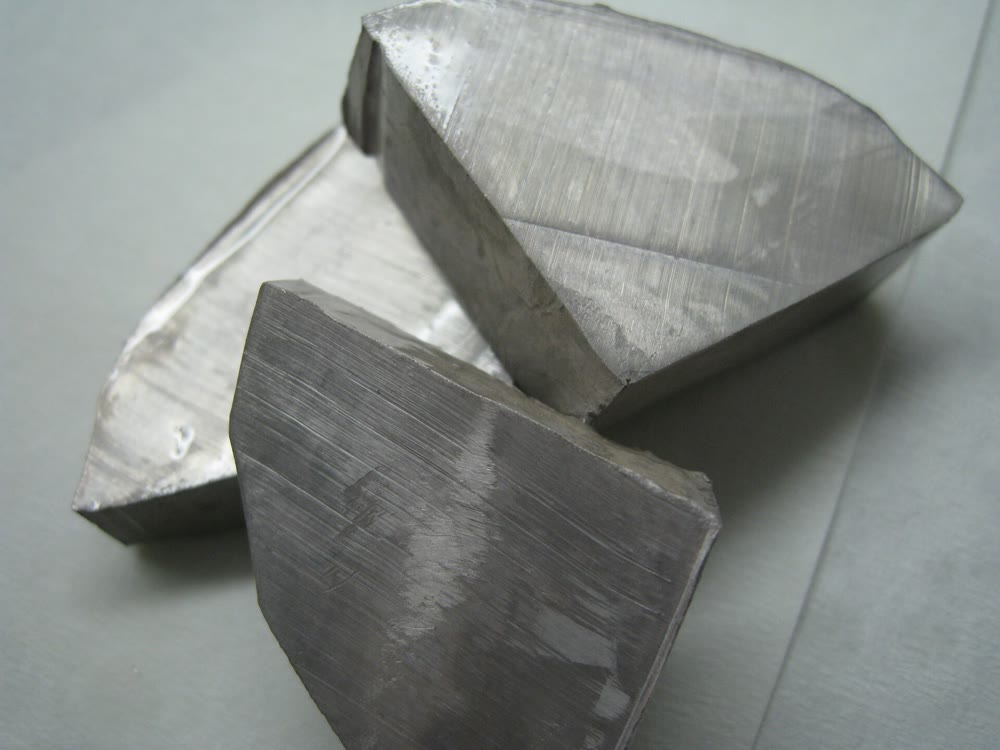
\includegraphics[width=\linewidth,height=4.4cm,keepaspectratio]{images/book1/sodium.jpg}

{\small 钠，一种\omterm{def:g10:electron-shells:family}{碱金属}，用刀切开后：新鲜时柔软、呈银白色，
在\omterm{def:g4:air-a-mixture-of-gases:air}{空气}中会立即失去光泽。照片：Dnn87，CC BY-SA 3.0。}
\end{minipage}\hfill
\begin{minipage}[b]{0.48\linewidth}\centering
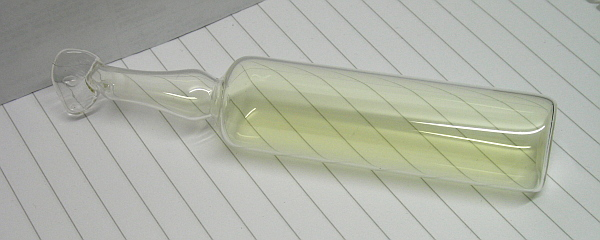
\includegraphics[width=\linewidth,height=4.4cm,keepaspectratio]{images/book1/chlorine-ampoule.jpg}

{\small 氯，一种\omterm{def:g10:electron-shells:family}{卤素}：黄绿色气体，此处
密封于玻璃安瓿瓶中。照片：W.~Oelen，CC BY-SA 3.0。}
\end{minipage}
\end{omfigure}

\begin{inthelab}[钠与水]
教师在防护屏后，将一小块米粒大小的钠
投入一大碗水中。钠漂浮于水面，熔化成一个发亮的小球，并
四处游动、嘶嘶作响，直至消失；放出的气体是氢气，
余下的水呈碱性。
\end{inthelab}

\begin{safety}{\ghs[0.75cm]{GHS02}\ghs[0.75cm]{GHS05}\quad\ghs[0.75cm]{GHS03}\ghs[0.75cm]{GHS06}}
% ledger: ghs:Na, ghs:Cl2
钠：与水反应放出易燃的氢气（GHS02），造成严重
灼伤（GHS05）。氯：氧化性气体（GHS03），吸入有毒
（GHS06），亦具刺激性，对水生生物毒性很大。两者均
仅由教师操作。
\end{safety}

\section{稳定离子与稀有气体规则}

\begin{definition}[二隅规则与八隅规则]\label{def:g10:electron-shells:octet}
\omterm{def:g10:electron-shells:family}{稀有气体}的最外\omterm{def:g10:electron-shells:configuration}{电子层}已充满，几乎不发生反应，其
\omterm{def:g10:electron-shells:configuration}{电子排布}特别稳定。前几种元素的\omterm{def:g7:atoms-and-molecules:atom}{原子}形成
\omterm{def:g9:ions:ion}{离子}时，通过得到或失去\omterm{def:g9:inside-the-atom:nucleus}{电子}，使其\omterm{def:g10:electron-shells:configuration}{电子排布}达到
最近\omterm{def:g10:electron-shells:family}{稀有气体}的\omterm{def:g10:electron-shells:configuration}{电子排布}：对于最轻的\omterm{def:g7:atoms-and-molecules:atom}{原子}，第 1 层有 2 个\omterm{def:g9:inside-the-atom:nucleus}{电子}，与氦相同，
即\emph{二隅规则}\index{二隅规则}；其他\omterm{def:g7:atoms-and-molecules:atom}{原子}则最外层
有 8 个\omterm{def:g9:inside-the-atom:nucleus}{电子}，与氖或氩相同，即
\emph{八隅规则}\index{八隅规则}。
\end{definition}

\begin{example}[规则预测的离子]\label{ex:g10:electron-shells:ions}
钠，$2.8.1$，失去唯一的\omterm{def:g10:electron-shells:valence}{价电子}：\ce{Na+}，$2.8$，与
氖相同。镁，$2.8.2$，失去 2 个：\ce{Mg^{2+}}。铝，$2.8.3$，
失去 3 个：\ce{Al^{3+}}。氯，$2.8.7$，得到 1 个：\ce{Cl-}，$2.8.8$，
与氩相同。氧，$2.6$，得到 2 个：\ce{O^{2-}}。硫，$2.8.6$：
\ce{S^{2-}}。锂，$2.1$，失去 1 个，保留 $2$，与氦相同：
\ce{Li+}。
\end{example}

\begin{omfigure}
\begin{tikzpicture}[font=\small]
  \foreach \x/\nm/\cfg/\col in {0/{Na}/{$1\mathrm{s}^2\,2\mathrm{s}^2\,2\mathrm{p}^6\,3\mathrm{s}^1$}/omDef,
      5.8/{\ce{Na+}}/{$1\mathrm{s}^2\,2\mathrm{s}^2\,2\mathrm{p}^6$}/omProp,
      11.0/{Ne}/{$1\mathrm{s}^2\,2\mathrm{s}^2\,2\mathrm{p}^6$}/gray} {
    \node[draw=\col, fill=\col!6, rounded corners=2pt, align=center, text width=3.4cm]
      at (\x,0) {\textbf{\nm}\\ \cfg};
  }
  \draw[->, thick, omProp] (2.0,0) -- (3.8,0) node[midway, above, font=\footnotesize] {失去 1 个 \ce{e-}};
  \node at (8.4,0) {$=$};
  \node[font=\footnotesize, align=center] at (8.4,-0.75) {相同 \\ 电子排布};
\end{tikzpicture}

{\small 钠\omterm{def:g9:ions:ion}{离子}的\omterm{def:g10:electron-shells:configuration}{电子排布}与最近的\omterm{def:g10:electron-shells:family}{稀有气体}
氖相同。}
\end{omfigure}

\begin{remark}[规则的局限]\label{rem:g10:electron-shells:limits}
该规则较好地适用于前二十种元素及其简单\omterm{def:g9:ions:ion}{离子}。
许多元素（如铁，\ce{Fe^{2+}} 和 \ce{Fe^{3+}}）不遵循该规则，
其原因及对\omterm{def:g9:inside-the-atom:nucleus}{电子}更好的描述，均在
本科一年级分册中给出。
\end{remark}

\section{练习}

\begin{exercise}[$\star$]\label{exo:g10:electron-shells:1}
写出碳（$Z = 6$）、氮（$Z = 7$）
和镁（$Z = 12$）的\omterm{def:g10:electron-shells:configuration}{电子排布}。
\end{exercise}

\begin{exercise}[$\star$]\label{exo:g10:electron-shells:2}
碳、氮和镁分别有多少个\omterm{def:g10:electron-shells:valence}{价电子}？
\end{exercise}

\begin{exercise}[$\star$]\label{exo:g10:electron-shells:3}
\omterm{def:g10:electron-shells:configuration}{电子排布}为
$1\mathrm{s}^2\,2\mathrm{s}^2\,2\mathrm{p}^6\,3\mathrm{s}^2\,3\mathrm{p}^3$ 的元素位于第几周期、第几族？
\end{exercise}

\begin{exercise}[$\star$]\label{exo:g10:electron-shells:4}
写出本章的三个\omterm{def:g10:electron-shells:family}{元素族}，并各举两种元素。
\end{exercise}

\begin{exercise}[$\star$]\label{exo:g10:electron-shells:5}
叙述\omterm{def:g10:electron-shells:octet}{八隅规则}。
\end{exercise}

\begin{exercise}[$\star\star$]\label{exo:g10:electron-shells:6}
利用\omterm{def:g10:electron-shells:family}{稀有气体}规则，写出钾（$Z = 19$）和
氟（$Z = 9$）分别形成的\omterm{def:g9:ions:ion}{离子}，并写出它们的\omterm{def:g10:electron-shells:configuration}{电子排布}。
\end{exercise}

\begin{exercise}[$\star\star$]\label{exo:g10:electron-shells:7}
某元素的第三\omterm{def:g10:electron-shells:configuration}{电子层}上有 2 个\omterm{def:g9:inside-the-atom:nucleus}{电子}，且第三\omterm{def:g10:electron-shells:configuration}{电子层}是其
最外\omterm{def:g10:electron-shells:configuration}{电子层}。写出该元素的\omterm{def:g10:electron-shells:configuration}{电子排布}、\omterm{def:g9:inside-the-atom:atomic-number}{原子序数}和名称。
\end{exercise}

\begin{exercise}[$\star\star$]\label{exo:g10:electron-shells:8}
利用稳定\omterm{def:g9:ions:ion}{离子}，写出镁与氯形成的
\omterm{def:g9:ions:ionic-compound}{离子化合物}的化学式，再写出铝与氧形成的\omterm{def:g9:ions:ionic-compound}{离子化合物}的化学式。
\end{exercise}

\begin{exercise}[$\star\star$]\label{exo:g10:electron-shells:9}
观察前二十号元素的表。哪些元素具有
与氧相同的\omterm{def:g10:electron-shells:valence}{价电子}数？
\end{exercise}

\begin{exercise}[$\star\star$]\label{exo:g10:electron-shells:10}
为什么氖与钠、氯不同，在\omterm{def:g7:chemical-reactions:reaction}{化学
反应}中不形成\omterm{def:g9:ions:ion}{离子}？
\end{exercise}

\begin{exercise}[$\star\star$]\label{exo:g10:electron-shells:11}
\omterm{def:g9:ions:ion}{离子} \ce{X^{2+}} 具有氩的\omterm{def:g10:electron-shells:configuration}{电子排布}。求 $X$。
\end{exercise}

\begin{exercise}[$\star\star\star$]\label{exo:g10:electron-shells:12}
氦有 2 个\omterm{def:g10:electron-shells:valence}{价电子}，却位于第 18 族，而非第 2 族。
请利用其\omterm{def:g10:electron-shells:configuration}{电子排布}加以解释。
\end{exercise}

\begin{exercise}[$\star\star\star$]\label{exo:g10:electron-shells:13}
钾与水的反应比钠更为剧烈。利用\omterm{def:g10:electron-shells:valence}{价电子}
与\omterm{def:g9:inside-the-atom:nucleus}{原子核}的距离，说明原因。
\end{exercise}

\begin{exercise}[$\star\star\star$]\label{exo:g10:electron-shells:14}
写出 \ce{S^{2-}}、\ce{Cl-}、\ce{K+} 和
\ce{Ca^{2+}} 的\omterm{def:g10:electron-shells:configuration}{电子排布}。它们有什么共同之处？
\end{exercise}

\begin{exercise}[$\star\star\star$]\label{exo:g10:electron-shells:15}
第 3 周期的某元素形成\omterm{def:g9:ions:ion}{离子} \ce{Y^{3-}}。
求该元素所在的族、其\omterm{def:g10:electron-shells:configuration}{电子排布}和名称。
\end{exercise}

\section{问题：红宝石、蓝宝石与刚玉}

\begin{problem}[{周末问题——宝石背后的电子：从两种电子排布到
一克中转移的电子数}]
\label{pb:g10:electron-shells:1}
红宝石和蓝宝石是刚玉的宝石形态，刚玉是一种
由铝和氧组成的\omterm{def:g9:ions:ionic-compound}{离子化合物}；微量的其他\omterm{def:g9:periodic-table-first-look:metal}{金属}使它们呈现颜色。
刚玉的硬度很高，几乎能划伤任何物质，粉末状的刚玉
可用于抛光透镜。取一个\omterm{def:g9:inside-the-atom:proton}{核子}的质量为
\qty{1.67e-27}{kg}；铝-27 含有 27 个\omterm{def:g9:inside-the-atom:proton}{核子}，氧-16 含有 16 个\omterm{def:g9:inside-the-atom:proton}{核子}。

\medskip
\noindent\textbf{第一部分——\omterm{def:g7:atoms-and-molecules:atom}{原子}。}
\begin{enumerate}
  \item 求铝\omterm{def:g7:atoms-and-molecules:atom}{原子}（$Z = 13$）和
        氧\omterm{def:g7:atoms-and-molecules:atom}{原子}（$Z = 8$）的\omterm{def:g9:inside-the-atom:proton}{质子}数与\omterm{def:g9:inside-the-atom:nucleus}{电子}数。
  \item 写出它们的\omterm{def:g10:electron-shells:configuration}{电子排布}。
  \item 每种\omterm{def:g7:atoms-and-molecules:atom}{原子}各有多少个\omterm{def:g10:electron-shells:valence}{价电子}？各位于
        第几周期、第几族？
  \item 铝是\omterm{def:g9:periodic-table-first-look:metal}{金属}还是\omterm{def:g9:periodic-table-first-look:metal}{非金属}？氧呢？
\end{enumerate}

\medskip
\noindent\textbf{第二部分——\omterm{def:g9:ions:ion}{离子}。}
\begin{enumerate}[resume]
  \item 利用\omterm{def:g10:electron-shells:octet}{八隅规则}，铝形成何种\omterm{def:g9:ions:ion}{离子}？写出其
        \omterm{def:g10:electron-shells:configuration}{电子排布}。
  \item 氧形成何种\omterm{def:g9:ions:ion}{离子}？写出其\omterm{def:g10:electron-shells:configuration}{电子排布}。
  \item 哪种\omterm{def:g10:electron-shells:family}{稀有气体}与这两种\omterm{def:g9:ions:ion}{离子}的\omterm{def:g10:electron-shells:configuration}{电子排布}相同？
  \item 一个铝\omterm{def:g7:atoms-and-molecules:atom}{原子}失去多少个\omterm{def:g9:inside-the-atom:nucleus}{电子}，一个氧\omterm{def:g7:atoms-and-molecules:atom}{原子}
        得到多少个\omterm{def:g9:inside-the-atom:nucleus}{电子}？
\end{enumerate}

\medskip
\noindent\textbf{第三部分——化学式。}
\begin{enumerate}[resume]
  \item 求由这些\omterm{def:g9:ions:ion}{离子}组成的电中性化合物刚玉的化学式。
  \item 在一个化学式单位中，铝\omterm{def:g7:atoms-and-molecules:atom}{原子}失去多少个\omterm{def:g9:inside-the-atom:nucleus}{电子}？
        氧\omterm{def:g7:atoms-and-molecules:atom}{原子}得到多少个\omterm{def:g9:inside-the-atom:nucleus}{电子}？
  \item 为什么这两个数必须相等？
  \item 红宝石中含有微量的铬\omterm{def:g9:ions:ion}{离子} \ce{Cr^{3+}}，它替代了
        部分 \ce{Al^{3+}} \omterm{def:g9:ions:ion}{离子}。为什么 \ce{Cr^{3+}} \omterm{def:g9:ions:ion}{离子}
        能够替代 \ce{Al^{3+}} \omterm{def:g9:ions:ion}{离子}而不破坏电荷平衡？
\end{enumerate}

\medskip
\noindent\textbf{第四部分——一克刚玉。}
\begin{enumerate}[resume]
  \item 一个刚玉化学式单位中含有多少个\omterm{def:g9:inside-the-atom:proton}{核子}？
  \item 计算一个化学式单位的质量（忽略\omterm{def:g9:inside-the-atom:nucleus}{电子}）。
  \item 在 \qty{1}{g} 刚玉中含有多少个化学式单位？
  \item 这些化学式单位中含有多少个 \ce{Al^{3+}} \omterm{def:g9:ions:ion}{离子}和 \ce{O^{2-}} \omterm{def:g9:ions:ion}{离子}？
  \item 第 14 题中为什么可以忽略\omterm{def:g9:inside-the-atom:nucleus}{电子}？
  \item 有多少个\omterm{def:g9:inside-the-atom:nucleus}{电子}从铝转移到氧，以制成
        \qty{1}{g} 刚玉？
\end{enumerate}
\end{problem}
